\part{Transformers}
\title{Transformers}  
\date{}  
\frame{\titlepage} 

%%%%%%%%%%%%%%%%%%%%%%%%%%%%%%%%%%%%%%%%%%%%%%%%%%%%%%%%%%%%%
%% Transformer definition %%
%%%%%%%%%%%%%%%%%%%%%%%%%%%%%%%%%%%%%%%%%%%%%%%%%%%%%%%%%%%%%
\begin{frame}
	\frametitle{Transformer definition}
    \begin{columns}
		\begin{column}{0.65\textwidth}
            \begin{varblock}{Transformer}
                A transformer is a static device that transfers electrical energy between two or more circuits through electromagnetic induction. It converts the AC voltage levels between inputs and outputs.   
            \end{varblock}
            \begin{itemize}
                \item While a transformer is sometimes called a ``static~machine'', it does not meet the formal definition of an electrical machine (compare first chapter).
                \item However, transformers share some working principles with electrical machines and are also often used as components of electrical power systems including drives.
            \end{itemize}
		\end{column}
        \hfill
		\begin{column}{0.35\textwidth}
			\begin{figure}
				\centering
				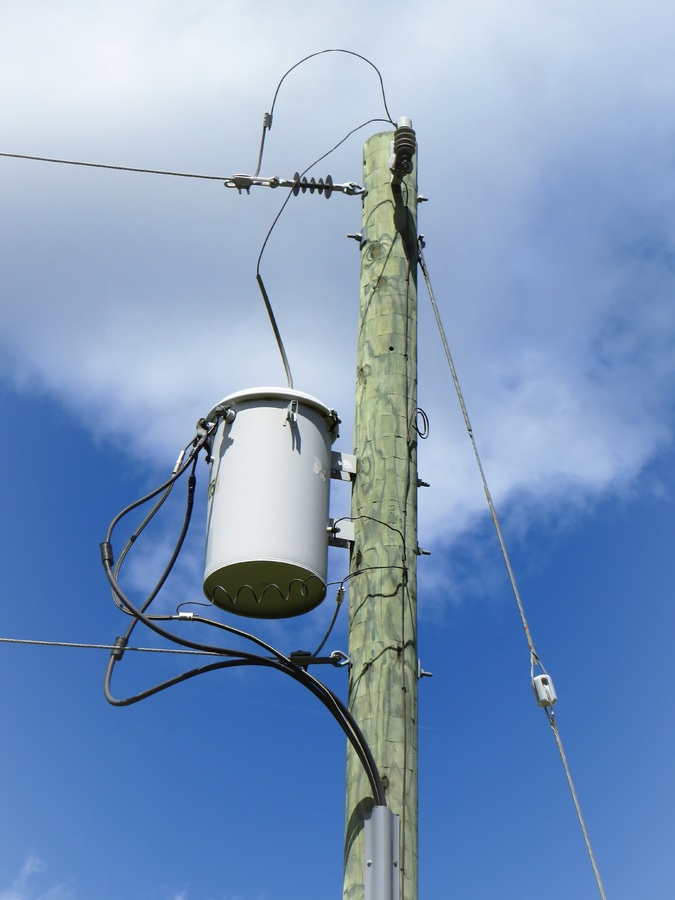
\includegraphics[width=0.75\textwidth]{fig/lec04/Transformer_rural_pole.jpg}
				\caption{Transformer integrated at a utility pole (source: \href{https://pxhere.com/en/photo/795672}{pxhere.com}, public domain)}
			\end{figure}
		\end{column}
		\end{columns}
\end{frame}

%%%%%%%%%%%%%%%%%%%%%%%%%%%%%%%%%%%%%%%%%%%%%%%%%%%%%%%%%%%%%
%% Examples of transformers %%
%%%%%%%%%%%%%%%%%%%%%%%%%%%%%%%%%%%%%%%%%%%%%%%%%%%%%%%%%%%%%
\begin{frame}
	\frametitle{Examples of transformers}
	\begin{figure}
		\centering
		\begin{subfigure}[b]{0.49\textwidth}
			\centering
			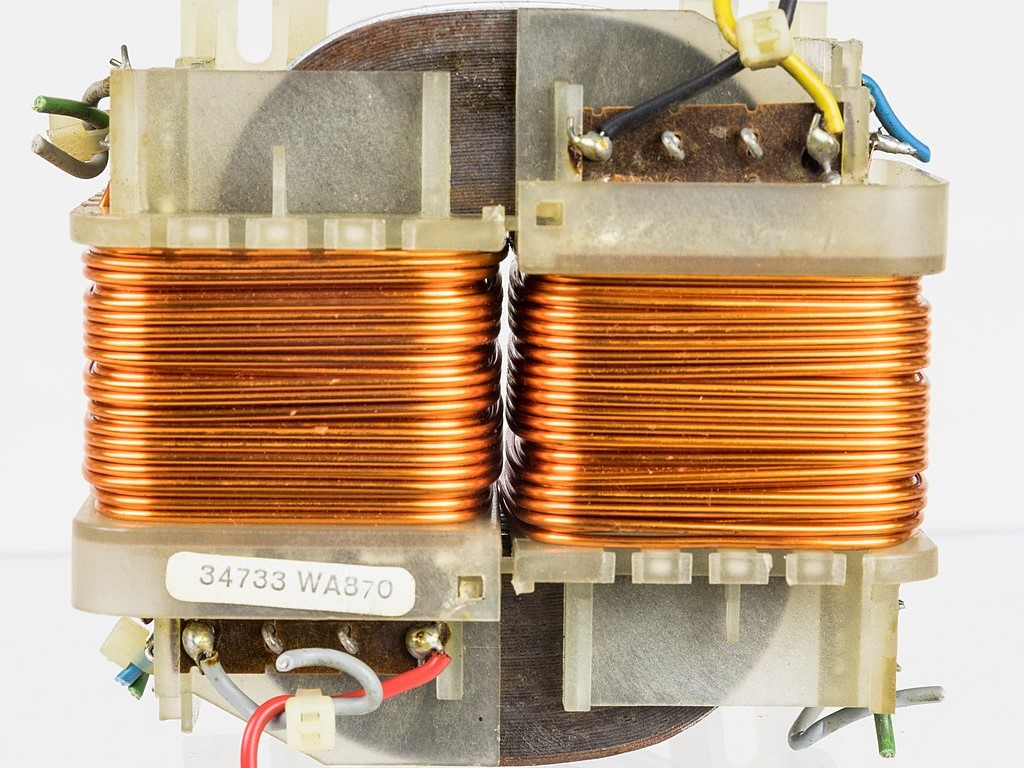
\includegraphics[width=0.45\textwidth]{fig/lec04/Power_supply_transformer.jpg}
			\caption{Power supply transformer (source: \href{https://commons.wikimedia.org/wiki/File:Philips_N4422_-_power_supply_transformer-2098.jpg}{Wikimedia Commons}, R.~Spekking, \href{https://creativecommons.org/licenses/by-sa/4.0/deed}{CC BY-SA 4.0})}
		\end{subfigure}
		\hfill
		\begin{subfigure}[b]{0.49\textwidth}
			\centering
			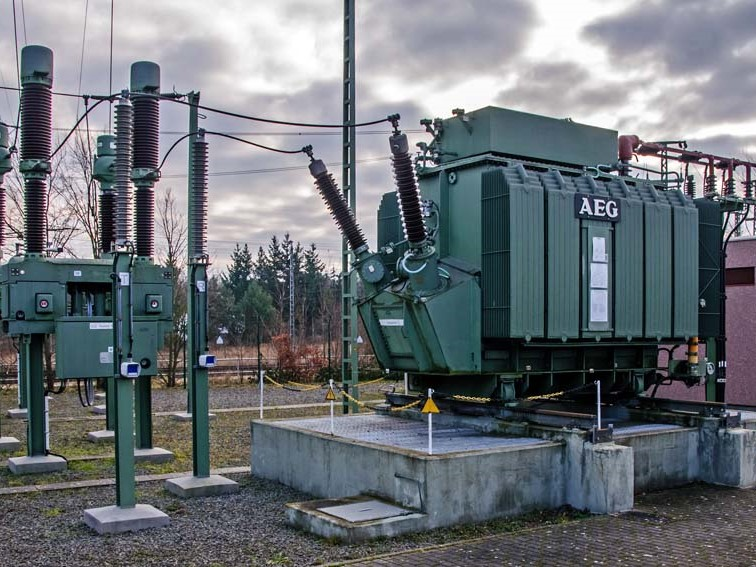
\includegraphics[width=0.45\textwidth]{fig/lec04/Single_phase_transformer.jpg}
			\caption{Single-phase transformer (source: \href{https://commons.wikimedia.org/wiki/File:DB_Unterwerk_Güsen,_Trafo_p.jpg}{Wikimedia Commons}, Georg, \href{https://creativecommons.org/licenses/by-sa/4.0/deed.en}{CC BY-SA 4.0})}
		\end{subfigure}
		\\
		\begin{subfigure}[b]{0.49\textwidth}
			\centering
			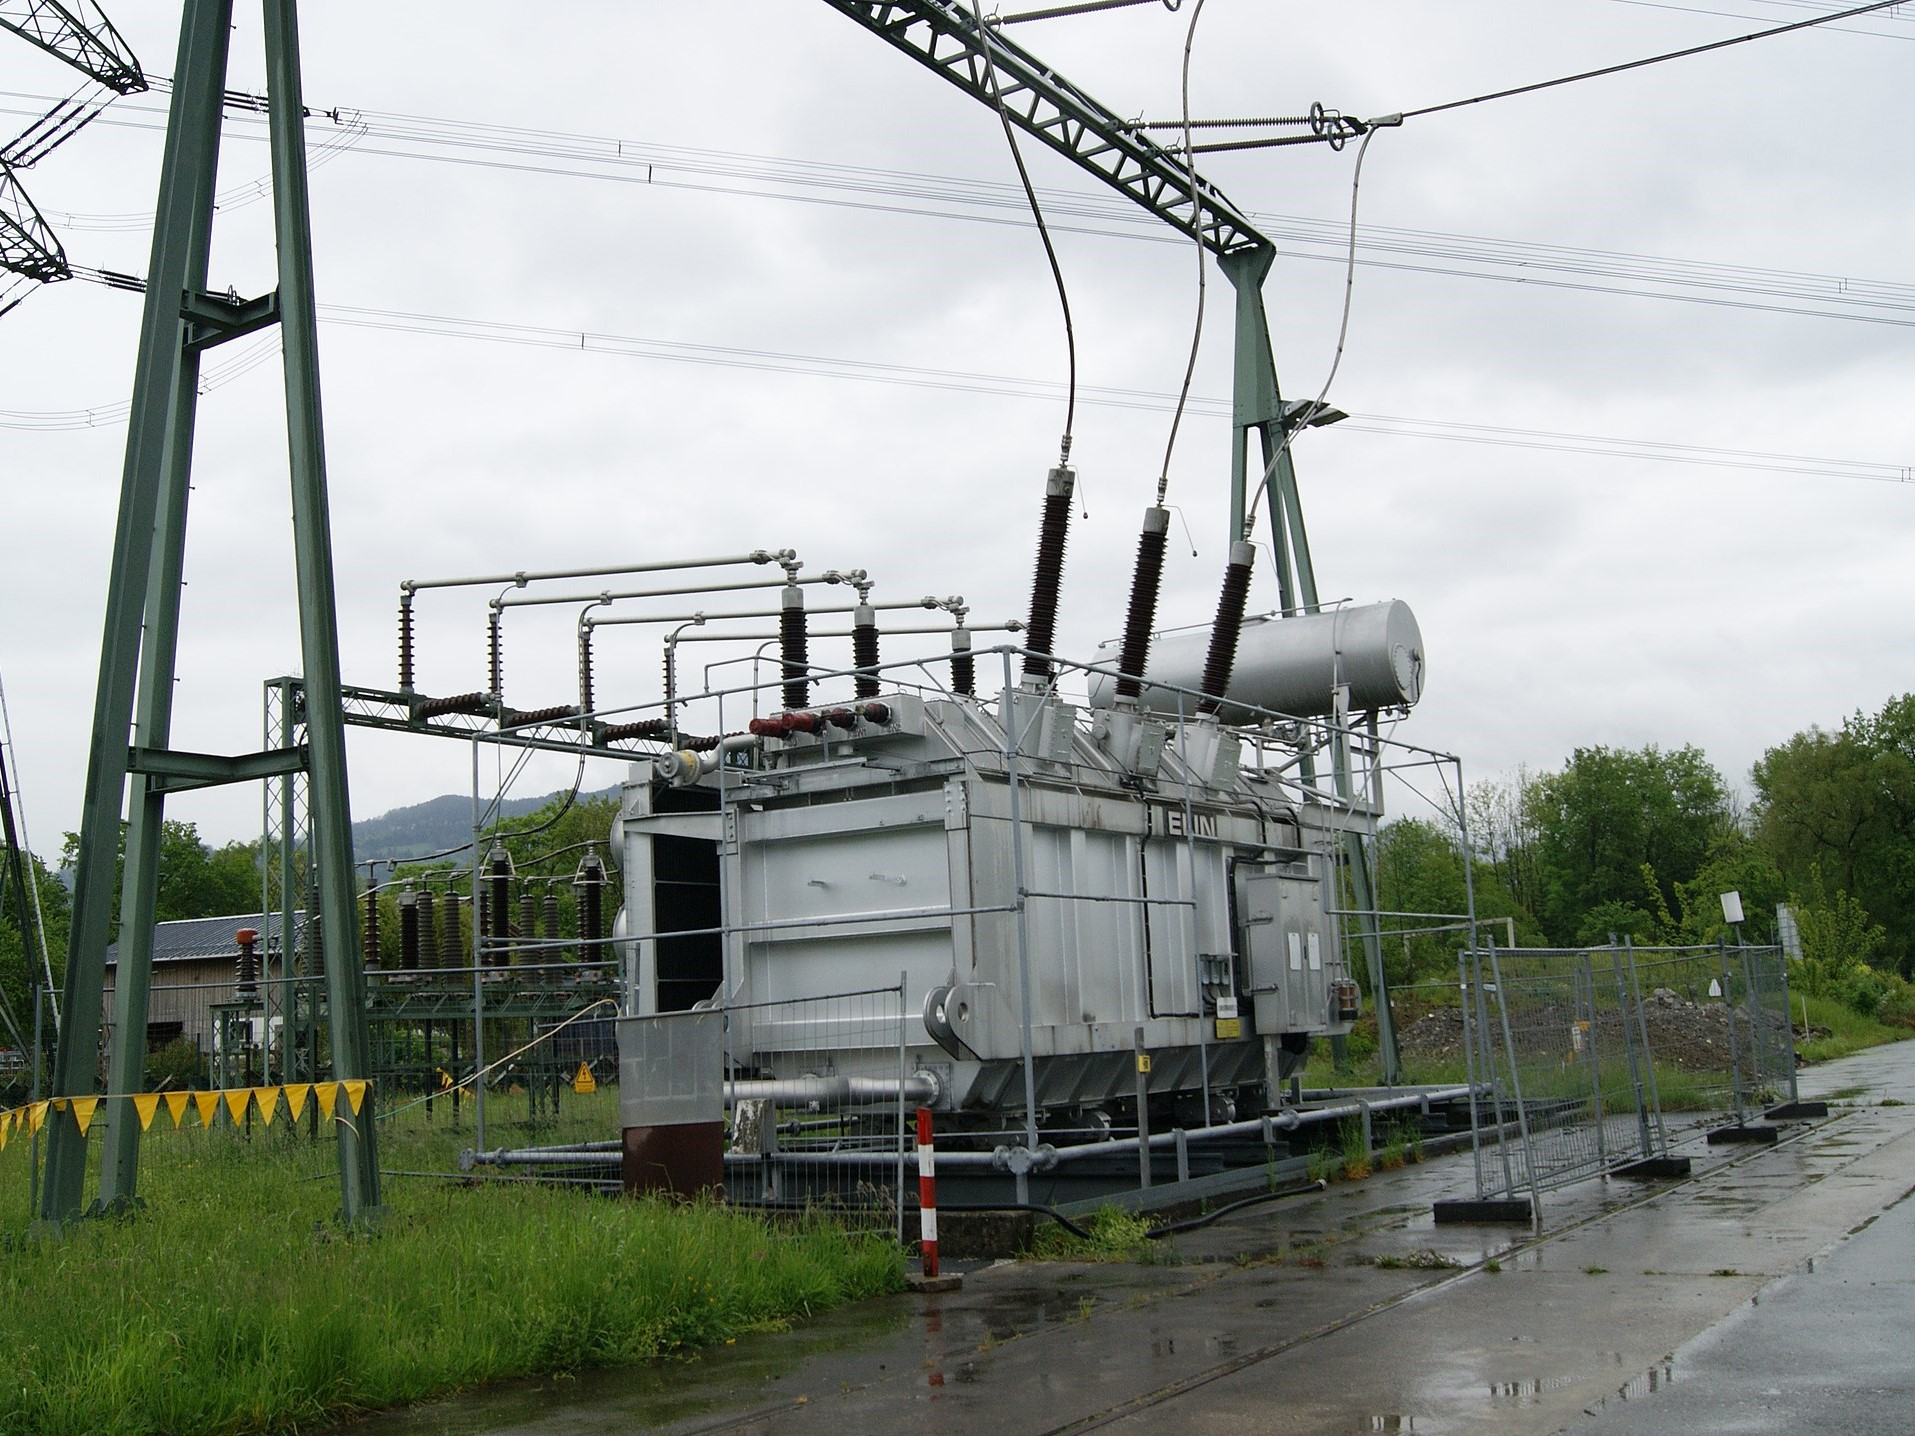
\includegraphics[width=0.45\textwidth]{fig/lec04/Three_phase_transformer.jpg}
			\caption{Three-phase transformer (source: \href{https://commons.wikimedia.org/wiki/File:Dornbirn-Umspannwerk_Werben-110kV_FS6-Anlage_Trafo_Elin_220-110kV-01ASD.jpg}{Wikimedia Commons}, Asurnipal, \href{https://creativecommons.org/licenses/by-sa/4.0/deed.en}{CC BY-SA 4.0})}
		\end{subfigure}
		\hfill
		\begin{subfigure}[b]{0.49\textwidth}
			\centering
			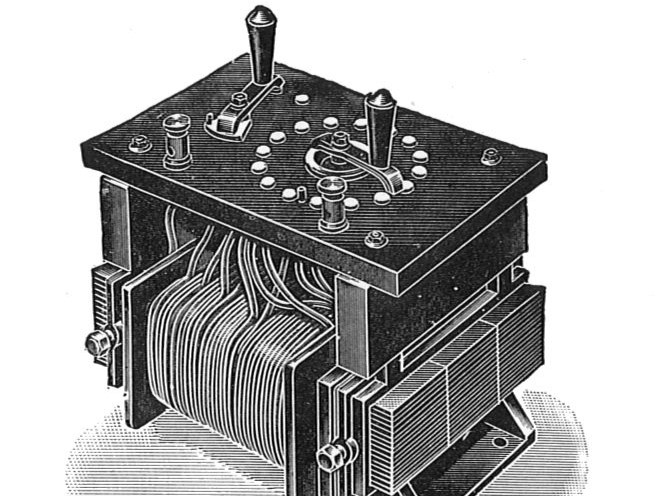
\includegraphics[width=0.45\textwidth]{fig/lec04/Tapped_transformer.jpg}
			\caption{Variable tapped transformer (source: \href{https://commons.wikimedia.org/wiki/File:Variable-tap_regulating_transformer_(Rankin_Kennedy,_Electrical_Installations,_Vol_II,_1909).jpg}{Wikimedia Commons}, public domain)}
		\end{subfigure}
		\caption*{Examples of transformers} 
        \label{fig:examples_transformers}
	\end{figure}
\end{frame}

%%%%%%%%%%%%%%%%%%%%%%%%%%%%%%%%%%%%%%%%%%%%%%%%%%%%%%%%%%%%%
%% Electromagnetic modeling of the single-phase transformer %%
%%%%%%%%%%%%%%%%%%%%%%%%%%%%%%%%%%%%%%%%%%%%%%%%%%%%%%%%%%%%%
\begin{frame}
	\frametitle{Electromagnetic modeling of the single-phase transformer}
    \begin{columns}
		\begin{column}{0.45\textwidth}
            Recap from \eqref{eq:flux_linkage_matrix_transformer}: for some given current $\bm{i}$, the flux linkages $\bm{\psi}$ in the transformer windings are
			\begin{equation*}
				\bm{\psi} = \begin{bmatrix} \psi_1 \\ \psi_2 \end{bmatrix} = \begin{bmatrix} L_1 & M \\ M & L_2 \end{bmatrix} \begin{bmatrix} i_1 \\ i_2 \end{bmatrix} = \bm{L}\bm{i}
			\end{equation*}
			where $L_1$ and $L_2$ are the self-inductances of the primary and secondary winding, respectively, and $M$ is the mutual inductance.
			\\[1em]
			Note: The above equation is an algebraic relation, that is, it is valid for any time instant $t$ and applies to both AC and DC excitation of the transformer. 
		\end{column}
        \hfill
		\begin{column}{0.525\textwidth}
			\begin{figure}
				\centering
				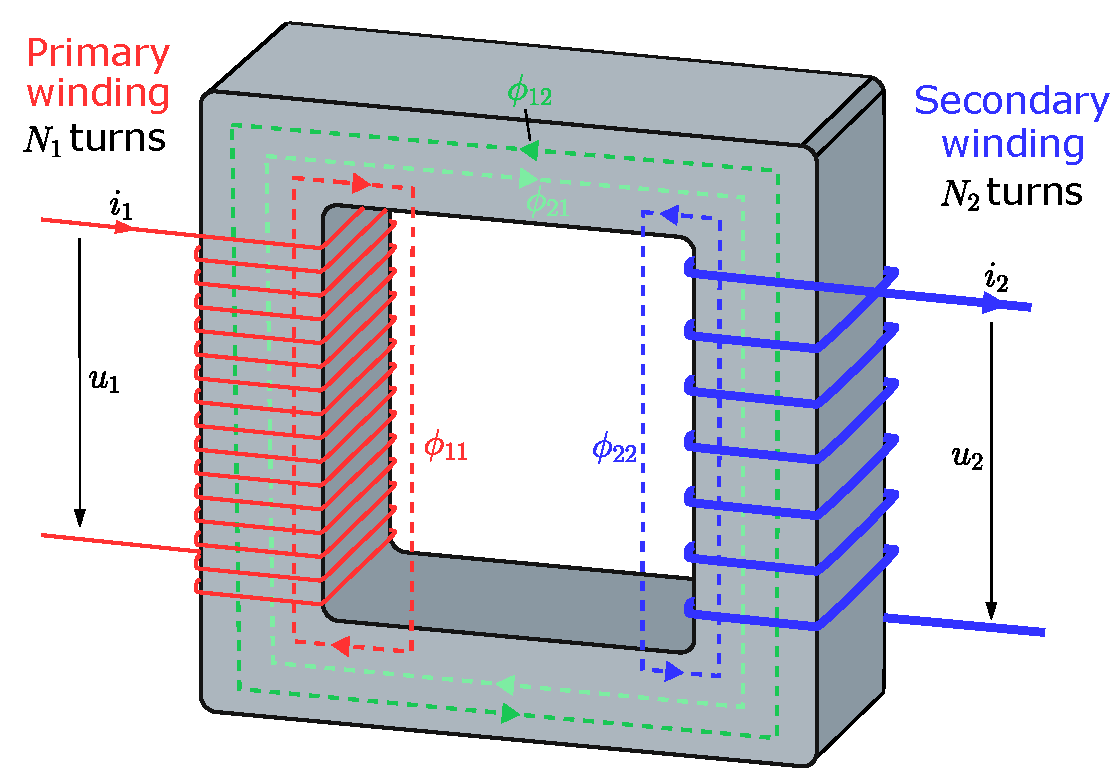
\includegraphics[height=0.575\textheight]{fig/lec02/Transformer3d_col3.pdf}
			\end{figure}
		\end{column}
		\end{columns}
\end{frame}

%%%%%%%%%%%%%%%%%%%%%%%%%%%%%%%%%%%%%%%%%%%%%%%%%%%%%%%%%%%%%
%% Dynamic modeling of the single-phase transformer %%
%%%%%%%%%%%%%%%%%%%%%%%%%%%%%%%%%%%%%%%%%%%%%%%%%%%%%%%%%%%%%
\begin{frame}
	\frametitle{Dynamic modeling of the single-phase transformer}
		The dynamic transformer behavior can be represented by the ECD in \figref{fig:General_transformer_ECD}, which also considers the internal resistances of the windings. Applying Faraday's law, the resulting differential equations are:
		\begin{align}
			u_1(t) = R_1 i_1(t) + \frac{\mathrm{d}\psi_1(t)}{\mathrm{d}t}, \qquad u_2(t) = R_2 i_2(t) + \frac{\mathrm{d}\psi_2(t)}{\mathrm{d}t}. \label{eq:transformer_differential_equations}
		\end{align}
		Inserting \eqref{eq:flux_linkage_matrix_transformer} delivers:
		\begin{align}
			u_1(t) = R_1 i_1(t) + L_1 \frac{\mathrm{d}i_1(t)}{\mathrm{d}t} + M \frac{\mathrm{d}i_2(t)}{\mathrm{d}t}, \qquad
			u_2(t) = R_2 i_2(t) + L_2 \frac{\mathrm{d}i_2(t)}{\mathrm{d}t} + M \frac{\mathrm{d}i_1(t)}{\mathrm{d}t}. \label{eq:transformer_differential_equations_2}
		\end{align}
		
\begin{figure}
\begin{columns}
	\begin{column}{0.55\textwidth}
            \centering
            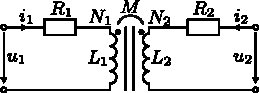
\includegraphics[width=0.8\textwidth]{fig/lec04/General_transformer_ECD.pdf}
    \end{column}
    \begin{column}{0.45\textwidth}
        \caption{\raggedright General equivalent circuit diagram (ECD) of a transformer (note: that both ports of the transformer are denoted in the load convention reference frame which is an arbitrary representation decision).}
		\label{fig:General_transformer_ECD}
    \end{column}
\end{columns}
\end{figure}
\end{frame}

%%%%%%%%%%%%%%%%%%%%%%%%%%%%%%%%%%%%%%%%%%%%%%%%%%%%%%%%%%%%%
%% Dynamic modeling of the single-phase transformer (cont.) %%
%%%%%%%%%%%%%%%%%%%%%%%%%%%%%%%%%%%%%%%%%%%%%%%%%%%%%%%%%%%%%
\begin{frame}
	\frametitle{Dynamic modeling of the single-phase transformer (cont.)}
		The model \eqref{eq:transformer_differential_equations_2} can be represented by the T-type ECD in \figref{fig:Transformer_T_ECD}. It may be noted that $L_1-M$ and $L_2-M$ can have negative values due to the model representation. 
		\\[1em]
		By rewritting \eqref{eq:transformer_differential_equations_2}, we can also write the dynamic transformer model in vector-matrix form:
		\begin{equation}
			\begin{bmatrix}	u_1(t)\\u_2(t) \end{bmatrix} = \bm{u}(t) = \begin{bmatrix} R_1 & 0 \\ 0 & R_2 \end{bmatrix} \begin{bmatrix} i_1(t)\\i_2(t) \end{bmatrix} + \begin{bmatrix} L_1 & M \\ M & L_2 \end{bmatrix} \frac{\mathrm{d}}{\mathrm{d}t} \begin{bmatrix} i_1(t)\\i_2(t) \end{bmatrix} = \bm{R}\bm{i}(t) + \bm{L}\frac{\mathrm{d}}{\mathrm{d}t}\bm{i}(t).  
			\label{eq:transformer_differential_equations_matrix_form}
		\end{equation}
\begin{figure}
\begin{columns}
	\begin{column}{0.55\textwidth}
            \centering
            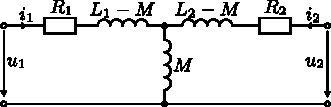
\includegraphics[width=0.9\textwidth]{fig/lec04/Transformer_T_ECD.pdf}
    \end{column}
    \begin{column}{0.45\textwidth}
        \caption{\raggedright T-type ECD of a transformer (note that the model \eqref{eq:transformer_differential_equations_matrix_form} assumes linear time-invariant (LTI) behavior, which among other effects neglects magnetic saturation).}
		\label{fig:Transformer_T_ECD}
    \end{column}
\end{columns}
\end{figure}
\end{frame}

%%%%%%%%%%%%%%%%%%%%%%%%%%%%%%%%%%%%%%%%%%%%%%%%%%%%%%%%%%%%%
%% Dynamic modeling of the single-phase transformer (cont.) %%
%%%%%%%%%%%%%%%%%%%%%%%%%%%%%%%%%%%%%%%%%%%%%%%%%%%%%%%%%%%%%
\begin{frame}
	\frametitle{Dynamic modeling of the single-phase transformer (cont.)}
		Rearranging \eqref{eq:transformer_differential_equations_matrix_form} gives the state-space representation of the transformer model
		\begin{equation}
			\frac{\mathrm{d}}{\mathrm{d}t}\bm{i}(t) = \bm{L}^{-1}\left(\bm{u}(t)-\bm{R}\bm{i}(t) \right)
			\label{eq:transformer_state_space_01}
		\end{equation}
		with
		$$ \renewcommand*{\arraystretch}{1.3} \bm{L}^{-1} = \frac{1}{L_1L_2 - M^2} \begin{bmatrix} L_2 & -M \\ -M & L_1 \end{bmatrix} = \frac{1}{\sigma} \begin{bmatrix} \frac{1}{L_1} &  \frac{-M}{L_1 L_2} \\ \frac{-M}{L_1 L_2} & \frac{1}{L_2} \end{bmatrix}.$$
		Above, $\sigma$ is the leakage coefficient defined as (compare also \eqref{eq:coupling_coefficient})
		\begin{equation}
			\sigma = \frac{L_1 L_2 -M^2}{L_1 L_2 } = 1 - \frac{M^2}{ L_1 L_2} = 1 - k^2 .
		\end{equation}
		Finally, the state-space representation of the transformer model is
		\begin{equation}
			\renewcommand*{\arraystretch}{1.3} 
			\frac{\mathrm{d}}{\mathrm{d}t}\bm{i}(t) = \begin{bmatrix} -\frac{R_1}{\sigma L_1} & \frac{R_2 M}{\sigma L_1 L_2} \\ \frac{R_1 M}{\sigma L_1 L_2} & -\frac{R_2}{\sigma L_1} \end{bmatrix} \bm{i}(t) + \begin{bmatrix} \frac{1}{\sigma L_1} & -\frac{M}{\sigma L_1 L_2} \\ -\frac{M}{\sigma L_1 L_2} & \frac{1}{\sigma L_2} \end{bmatrix} \bm{u}(t) = \bm{A} \bm{i}(t) + \bm{B} \bm{u}(t) .	 
			\label{eq:transformer_state_space_02}
		\end{equation}
\end{frame}

%%%%%%%%%%%%%%%%%%%%%%%%%%%%%%%%%%%%%%%%%%%%%%%%%%%%%%%%%%%%%
%% Steady-state of the single-phase transformer %%
%%%%%%%%%%%%%%%%%%%%%%%%%%%%%%%%%%%%%%%%%%%%%%%%%%%%%%%%%%%%%
\begin{frame}
	\frametitle{Steady-state modeling of the single-phase transformer}
		Assuming that the transformer operates in steady state and that all quantities are sinusoidal, the state-space model \eqref{eq:transformer_state_space_02} can be simplified and represented by complex phasors:
			$$x(t) = \hat{x} \cos(\omega_\mathrm{el} t+ \varphi_{\mathrm{x}}) = \mathrm{Re}\left\{\hat{x} e^{\iu (\omega_\mathrm{el} t + \varphi_{\mathrm{x}})}\right\}= \mathrm{Re}\left\{\underline{X} e^{\iu \omega_\mathrm{el} t}\right\}.$$
		From \eqref{eq:transformer_differential_equations_matrix_form} we recieve
		\begin{align}
			\bm{\underline{U}} = \begin{bmatrix} \underline{U}_1 \\ \underline{U}_2 \end{bmatrix} = \bm{R}\bm{\underline{I}} + \iu \omega_\mathrm{el} \bm{L}\bm{\underline{I}} = \bm{\underline{Z}}\, \bm{\underline{I} } = \begin{bmatrix} R_1 + \iu \omega_\mathrm{el} L_1 & \iu \omega_\mathrm{el} M \\ \iu \omega_\mathrm{el} M & R_2 + \iu \omega_\mathrm{el} L_2 \end{bmatrix} \begin{bmatrix} \underline{I}_1 \\ \underline{I}_2 \end{bmatrix}.
			\label{eq:transformer_steady_state_voltage_response}
		\end{align}
		For some given $\bm{\underline{U}}$ we can calculate the current phasors $\bm{\underline{I}}$ (i.e., the steady-state current response) by solving:
		\begin{align}
			\renewcommand*{\arraystretch}{1.3} 
			\bm{\underline{I}} = \bm{\underline{Z}}^{-1} \bm{\underline{U}} .
			\label{eq:transformer_steady_state_current_response}
		\end{align}
		Alternative scenarios can be also considered, e.g., defining $\underline{U}_1$ (input voltage) and $\underline{I}_2$ (load current) as given and solving for $\underline{I}_1$ and $\underline{U}_2$ by rearranging \eqref{eq:transformer_steady_state_voltage_response}. 
\end{frame}

%%%%%%%%%%%%%%%%%%%%%%%%%%%%%%%%%%%%%%%%%%%%%%%%%%%%%%%%%%%%%
%% Steady-state of the single-phase transformer (cont.) %%
%%%%%%%%%%%%%%%%%%%%%%%%%%%%%%%%%%%%%%%%%%%%%%%%%%%%%%%%%%%%%
\begin{frame}
	\frametitle{Steady-state modeling of the single-phase transformer (cont.)}
		Assuming that the transformer is not loaded ($I_2 = 0$) and that it is lossless ($R_1 = 0$), \eqref{eq:transformer_steady_state_voltage_response} simplifies to
		\begin{equation}
			\begin{bmatrix} \underline{U}_1 \\ \underline{U}_2 \end{bmatrix} = \begin{bmatrix} \iu \omega_\mathrm{el} L_1  \\ \iu \omega_\mathrm{el} M  \end{bmatrix} \underline{I}_1.
		\end{equation}
		The voltage transformation ratio in this case results in
		\begin{equation}
			\frac{U_1}{U_2} = \frac{\iu \omega_{\mathrm{el}} L_1 I_1}{\iu \omega_{\mathrm{el}} M I_1}  = \frac{L_1}{M}.
		\end{equation}
		Assuming further that the transformer is leakage-free ($L_{1,\sigma}=0$), the voltage transformation ratio simplifies to (compare also \eqref{eq:inductance_split})
		\begin{equation}
			\frac{U_1}{U_2} = \frac{L_1}{M} = \frac{\Lambda_{21}N_1^2}{\Lambda_{21}N_1 N_2} I_1 = \frac{N_1}{N_2}.
		\end{equation}
		Hence, this famous result is only valid for the abstract case of a lossless, leakage-free, and, unloaded transformer -- i.e., not applicable to real-world transformers.
\end{frame}

%%%%%%%%%%%%%%%%%%%%%%%%%%%%%%%%%%%%%%%%%%%%%%%%%%%%%%%%%%%%%
%% Transformation of the secondary side variables %%
%%%%%%%%%%%%%%%%%%%%%%%%%%%%%%%%%%%%%%%%%%%%%%%%%%%%%%%%%%%%%
\begin{frame}
	\frametitle{Transformation of the secondary side variables}
		Sometimes it can be helpful to (mathematically) transform the secondary side variables to ease the mathematical analysis. This can be done by introducing the transformation factor $\alpha$:
		\begin{equation}
			u_2' = \alpha u_2, \qquad i_2' = \frac{1}{\alpha} i_2.
		\end{equation}
		Here, $u_2'$ and $i_2'$ are the transformed secondary side voltage and current, respectively. The primary voltage equation reads
		\begin{equation}
			\begin{split}
			u_1(t) &= R_1 i_1(t) + L_1 \frac{\mathrm{d}i_1(t)}{\mathrm{d}t} + M \frac{\mathrm{d}i_2(t)}{\mathrm{d}t}  = R_1 i_1 (t)+ L_1 \frac{\mathrm{d}i_1(t)}{\mathrm{d}t}  + \alpha M \frac{\mathrm{d}i_2'(t)}{\mathrm{d}t}  \\&= R_1 i_1(t) + L_1 \frac{\mathrm{d}i_1(t)}{\mathrm{d}t} + M' \frac{\mathrm{d}i_2'(t)}{\mathrm{d}t}
		\end{split}
		\end{equation}
		with the transformed mutual inductance $M' = \alpha M$. 
\end{frame}

%%%%%%%%%%%%%%%%%%%%%%%%%%%%%%%%%%%%%%%%%%%%%%%%%%%%%%%%%%%%%
%% Transformation of the secondary side variables (cont.) %%
%%%%%%%%%%%%%%%%%%%%%%%%%%%%%%%%%%%%%%%%%%%%%%%%%%%%%%%%%%%%%
\begin{frame}
	\frametitle{Transformation of the secondary side variables (cont.)}
		Multiplying the secondary voltage equation with $\alpha$ gives 
		\begin{equation}
			\begin{split}
			\alpha  u_2(t)  &=  \alpha R_2 i_2(t) + \alpha L_2 \frac{\mathrm{d}i_2(t)}{\mathrm{d}t} + \alpha M \frac{\mathrm{d}i_1(t)}{\mathrm{d}t}\\
			\Leftrightarrow \quad u_2'(t) &= \alpha^2 R_2 i_2'(t) + \alpha^2 L_2 \frac{\mathrm{d}i_2'(t)}{\mathrm{d}t} + \alpha M \frac{\mathrm{d}i_1(t)}{\mathrm{d}t}\\
			\Leftrightarrow \quad u_2'(t) &=  R'_2 i_2'(t) + L'_2 \frac{\mathrm{d}i_2'(t)}{\mathrm{d}t} + M' \frac{\mathrm{d}i_1(t)}{\mathrm{d}t}
		\end{split}
		\end{equation}
		with the transformed resistance $R'_2 = \alpha^2 R_2$ and inductance $L'_2 = \alpha^2 L_2$.
		\begin{figure}
			\begin{columns}
				\begin{column}{0.64\textwidth}
						\centering
						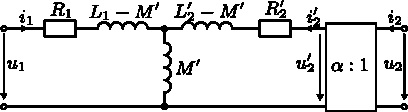
\includegraphics[width=0.99\textwidth]{fig/lec04/Transformer_T_ECD_gen_transf.pdf}
				\end{column}
				\begin{column}{0.35\textwidth}
					\caption{\raggedright T-type ECD of a transformer with transformed secondary side variables for some arbitrary transformation factor $\alpha$ (note that $k$ and $\sigma$ are transformation invariant.)}
					\label{fig:Transformer_T_ECD_gen_transf}
				\end{column}
			\end{columns}
		\end{figure}
\end{frame}

%%%%%%%%%%%%%%%%%%%%%%%%%%%%%%%%%%%%%%%%%%%%%%%%%%%%%%%%%%%%%
%% Transformation of the secondary side variables by the turn ratio %%
%%%%%%%%%%%%%%%%%%%%%%%%%%%%%%%%%%%%%%%%%%%%%%%%%%%%%%%%%%%%%
\begin{frame}
	\frametitle{Transformation of the secondary side variables by the turn ratio}
	With $$\alpha = N_1/N_2$$ as the transformation factor, we receive:
	\begin{equation}
		M' = (N_1/N_2)M = L_{1,\mathrm{m}}, \qquad L'_2 = (N_1^2/N_2^2) L_2
	\end{equation}
		with $L_{1,\mathrm{m}}$ being the primary magnetizing inductance, cf. \eqref{eq:inductance_split}. Moreover, we have
	\begin{equation}
		L_1 - M' = L_{1,\sigma}, \qquad L_2' - M'2 =  (N_1^2/N_2^2) L_{2,\sigma} = L'_{2,
		\sigma}
	\end{equation}
	with $L_{1,\sigma}$ and $L_{2,\sigma}$ being the leakage inductances of the primary and secondary winding. 
	\begin{figure}
		\begin{columns}
			\begin{column}{0.64\textwidth}
					\centering
					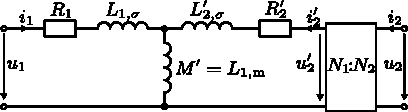
\includegraphics[width=0.99\textwidth]{fig/lec04/Transformer_T_ECD_turn_transf.pdf}
			\end{column}
			\begin{column}{0.35\textwidth}
				\caption{\raggedright T-type ECD of a transformer with $\alpha =N_1/N_2$ (note that all inductances within this model representation have a direct physical interpretation.)}
				\label{fig:Transformer_T_ECD_turn_transf}
			\end{column}
		\end{columns}
	\end{figure}	
\end{frame}

%%%%%%%%%%%%%%%%%%%%%%%%%%%%%%%%%%%%%%%%%%%%%%%%%%%%%%%%%%%%%
%% Transformation towards a single stray inductance %%
%%%%%%%%%%%%%%%%%%%%%%%%%%%%%%%%%%%%%%%%%%%%%%%%%%%%%%%%%%%%%
\begin{frame}
	\frametitle{Transformation towards a single stray inductance}
	With $$\alpha = M/L_2$$ as the transformation factor, we receive:
	\begin{equation}
		L'_2 - M' = \alpha^2 L_2 - \alpha M = L_{2,\sigma} = 0,
	\end{equation}
		that is, the secondary transformed leakage inductance is vanishing. Moreover, we have
	\begin{equation}
		L_1 - M' = L'_{1,\sigma}=\sigma L_1 , \qquad M'  = M^2 / L_2.
	\end{equation}
	With the alternative choice $\alpha = L_1/M$, the leakage inductance gets concentrated on the secondary side (not explicitly shown).
	\begin{figure}
		\begin{columns}
			\begin{column}{0.64\textwidth}
					\centering
					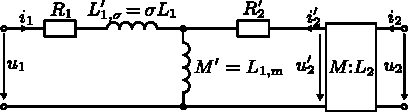
\includegraphics[width=0.99\textwidth]{fig/lec04/Transformer_T_ECD_stray_transf.pdf}
			\end{column}
			\begin{column}{0.35\textwidth}
				\caption{\raggedright T-type ECD of a transformer with $\alpha =M/L_2$}
				\label{fig:Transformer_T_ECD_stray_transf}
			\end{column}
		\end{columns}
	\end{figure}	
\end{frame}

%%%%%%%%%%%%%%%%%%%%%%%%%%%%%%%%%%%%%%%%%%%%%%%%%%%%%%%%%%%%%
%% Typical transformer core types %%
%%%%%%%%%%%%%%%%%%%%%%%%%%%%%%%%%%%%%%%%%%%%%%%%%%%%%%%%%%%%%
\begin{frame}
	\frametitle{Typical transformer core types}
	\begin{itemize}
		\item The core of a transformer typical build from laminated steel sheets (cf. \figref{fig:Eddy_currents_lamination}). Alternatively, sintered ferrite material is also used for high-frequency applications.
		\item To improve the coupling between primary and secondary winding, it is beneficial to place the windings around the same leg. Hence, the middle example in \figref{fig:Transformer_cores} will exhibit a larger leakage.
	\end{itemize}
	\begin{figure}
		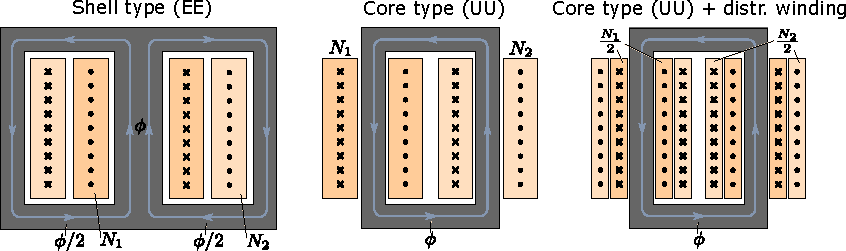
\includegraphics[width=0.9\textwidth]{fig/lec04/Transformer_cores.pdf}
		\caption{Examples of typical transformer core types}
		\label{fig:Transformer_cores}
	\end{figure}
\end{frame}

%%%%%%%%%%%%%%%%%%%%%%%%%%%%%%%%%%%%%%%%%%%%%%%%%%%%%%%%%%%%%
%% Typical transformer winding schemes %%
%%%%%%%%%%%%%%%%%%%%%%%%%%%%%%%%%%%%%%%%%%%%%%%%%%%%%%%%%%%%%
\begin{frame}
	\frametitle{Typical transformer winding schemes}
	\begin{itemize}
		\item The below examples show improving magnetic coupling (lower leakage) from left to right due to the reducing effective distance between the turns of the primary and secondary winding.
		\item Beyond these examples, various winding variations (e.g., a combination of the below schemes) are used to optimize the transformer design for specific applications. 
	\end{itemize}
	\vspace{0.5em}
	\begin{figure}
		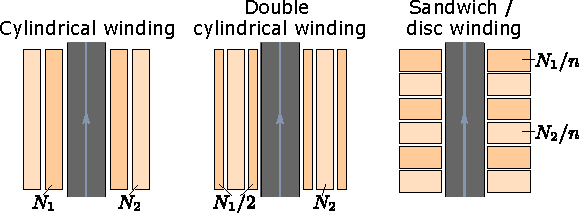
\includegraphics[width=0.7\textwidth]{fig/lec04/Transformer_winding_types.pdf}
		\caption{Examples of typical transformer winding schemes}
		\label{fig:Transformer_winding_types}
	\end{figure}
\end{frame}

%%%%%%%%%%%%%%%%%%%%%%%%%%%%%%%%%%%%%%%%%%%%%%%%%%%%%%%%%%%%%
%% Three-phase transformer %%
%%%%%%%%%%%%%%%%%%%%%%%%%%%%%%%%%%%%%%%%%%%%%%%%%%%%%%%%%%%%%
\begin{frame}
	\frametitle{Three-phase transformer}
	\begin{figure}
		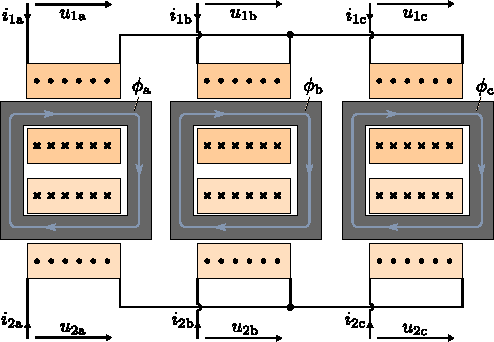
\includegraphics[width=0.6\textwidth]{fig/lec04/Three_phase_transformer_simple.pdf}
		\caption{Simple three-phase transformer with three independent single-phase transformers connected in star both on the primary and secondary side}
		\label{fig:Three_phase_transformer_simple}
	\end{figure}
\end{frame}

%%%%%%%%%%%%%%%%%%%%%%%%%%%%%%%%%%%%%%%%%%%%%%%%%%%%%%%%%%%%%
%% Three-phase transformer with five legs %%
%%%%%%%%%%%%%%%%%%%%%%%%%%%%%%%%%%%%%%%%%%%%%%%%%%%%%%%%%%%%%
\begin{frame}
	\frametitle{Three-phase transformer with five legs}
	\begin{figure}
		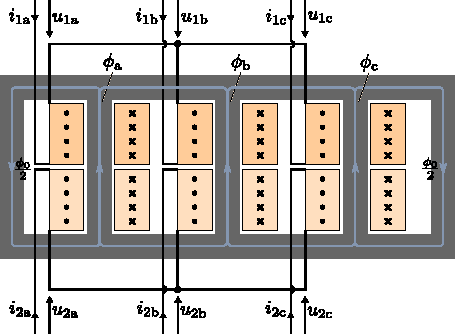
\includegraphics[height=0.75\textheight]{fig/lec04/Three_phase_transformer_5_legs.pdf}
		\caption{Three-phase five-leg transformer connected in star both on the primary and secondary side}
		\label{fig:Three_phase_transformer_5_legs}
	\end{figure}
\end{frame}


%%%%%%%%%%%%%%%%%%%%%%%%%%%%%%%%%%%%%%%%%%%%%%%%%%%%%%%%%%%%%
%% Three-phase transformer with five legs (cont.) %%
%%%%%%%%%%%%%%%%%%%%%%%%%%%%%%%%%%%%%%%%%%%%%%%%%%%%%%%%%%%%%
\begin{frame}
	\frametitle{Three-phase transformer with five legs (cont.)}
	Obviously, the three-phase five-leg design from \figref{fig:Three_phase_transformer_5_legs} can save space and material compared to the three independent single-phase transformers from \figref{fig:Three_phase_transformer_simple}. However, there might be a zero flux component
	\begin{equation}
		\phi_0(t) = \phi_\mathrm{a}(t) + \phi_\mathrm{b}(t) + \phi_\mathrm{c}(t)  
	\end{equation} 
	flowing via the winding-free legs. This zero flux component can be avoided if the primary and secondary side are connected both in star configuration
	$$ i_{1\mathrm{a}}(t)+i_{1\mathrm{b}}(t)+i_{1\mathrm{c}}(t)=0, \qquad i_{2\mathrm{a}}(t)+i_{2\mathrm{b}}(t)+i_{2\mathrm{c}}(t)=0$$
	and if the magnetic reluctances $\Lambda_\mathrm{m}$ of the three main legs are equal (i.e., symmetric design, no saturation):
	\begin{equation*}
		\phi_0 = \phi_\mathrm{a} + \phi_\mathrm{b} + \phi_\mathrm{c} = \Lambda_\mathrm{m} N_1 \left(i_{1\mathrm{a}}(t)+i_{1\mathrm{b}}(t)+i_{1\mathrm{c}}(t)\right)+\Lambda_\mathrm{m} N_2 \left(i_{2\mathrm{a}}(t)+i_{2\mathrm{b}}(t)+i_{2\mathrm{c}}(t)\right) = 0.
	\end{equation*}
\end{frame}

%%%%%%%%%%%%%%%%%%%%%%%%%%%%%%%%%%%%%%%%%%%%%%%%%%%%%%%%%%%%%
%% Three-phase transformer with three legs (double star connection) %%
%%%%%%%%%%%%%%%%%%%%%%%%%%%%%%%%%%%%%%%%%%%%%%%%%%%%%%%%%%%%%
\begin{frame}
	\frametitle{Three-phase transformer with three legs (double star connection)}
	\begin{columns}
		\begin{column}{0.4\textwidth}
           \begin{itemize}
				\item If the flux zero component $\phi_0$ can be avoided, a three-leg design as shown in \figref{fig:Three_phase_transformer_3_legs_star} can be used.
				\item However, if $\phi_0 \neq 0$ due to an asymmetric design, magnetic saturation or non-ideal symmetrical operation, the zero component will act as a stray field leaving the transformer core.
				\item This can lead to increased losses and electromagnetic interference.
			\end{itemize}
		\end{column}
        \hfill
		\begin{column}{0.6\textwidth}
			\begin{figure}
				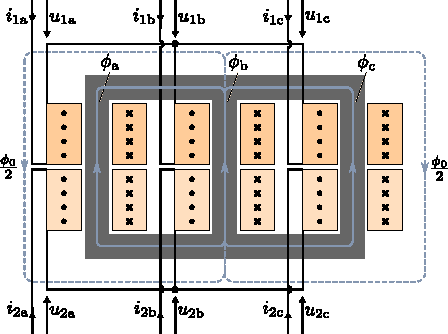
\includegraphics[height=0.7\textheight]{fig/lec04/Three_phase_transformer_3_legs_star.pdf}
				\caption{Three-phase three-leg transformer connected in star both on the primary and secondary side}
				\label{fig:Three_phase_transformer_3_legs_star}
			\end{figure}
		\end{column}
	\end{columns}
\end{frame}

%%%%%%%%%%%%%%%%%%%%%%%%%%%%%%%%%%%%%%%%%%%%%%%%%%%%%%%%%%%%%
%% Three-phase transformer with three legs (star-delta connection) %%
%%%%%%%%%%%%%%%%%%%%%%%%%%%%%%%%%%%%%%%%%%%%%%%%%%%%%%%%%%%%%
\begin{frame}
	\frametitle{Three-phase transformer with three legs (star-delta connection)}
	\begin{columns}
		\begin{column}{0.4\textwidth}
 			If the primary or secondary side is connected in delta configuration, this side can carry a zero sequence current:
			\begin{equation*}
				i_0 = \frac{1}{3}\left(i_\mathrm{a}(t) + i_\mathrm{b}(t) + i_\mathrm{c}(t)\right) \neq 0 .
			\end{equation*}
			This zero sequence current would not be visible in the phase conductors:
			\begin{equation}
				\begin{split}
					i_\mathrm{ab} &= i_\mathrm{a} - i_\mathrm{b}, \\ i_\mathrm{bc} &= i_\mathrm{b} - i_\mathrm{c},\\ i_\mathrm{ca} &= i_\mathrm{c} - i_\mathrm{a}.
				\end{split}
				\label{eq:zero_sequence_currents_phase_transformer}
			\end{equation}
		\end{column}
        \hfill
		\begin{column}{0.6\textwidth}
			\begin{figure}
				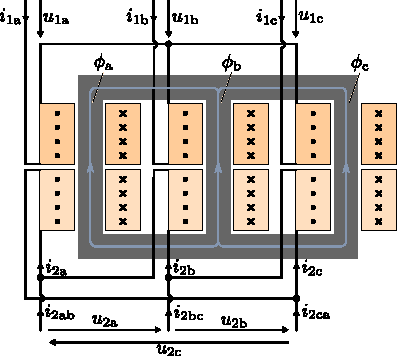
\includegraphics[height=0.7\textheight]{fig/lec04/Three_phase_transformer_3_legs_star_delta.pdf}
				\caption{Three-phase three-leg transformer connected in a star-delta configuration (delta on secondary is exemplary)}
				\label{fig:Three_phase_transformer_3_legs_star_delta}
			\end{figure}
		\end{column}
	\end{columns}
\end{frame}

%%%%%%%%%%%%%%%%%%%%%%%%%%%%%%%%%%%%%%%%%%%%%%%%%%%%%%%%%%%%%
%% Zero flux and zero current components in three-phase transformers %%
%%%%%%%%%%%%%%%%%%%%%%%%%%%%%%%%%%%%%%%%%%%%%%%%%%%%%%%%%%%%%
\begin{frame}
	\frametitle{Zero flux and zero current components in three-phase transformers}
	Based on \eqref{eq:zero_sequence_currents_phase_transformer} the winding currents on the delta side becomes
	\begin{equation}		
			i_\mathrm{a} = i_0 + \frac{1}{3}\left(i_\mathrm{ab}-i_\mathrm{ca}\right), \quad i_\mathrm{b} = i_0 + \frac{1}{3}\left(i_\mathrm{bc}-i_\mathrm{ab}\right), \quad i_\mathrm{c} = i_0 + \frac{1}{3}\left(i_\mathrm{ca}-i_\mathrm{bc}\right).
	\end{equation}
	If the secondary side is connected in delta, the zero sequence current will result from
	\begin{equation}
		\phi_0 = \phi_\mathrm{a} + \phi_\mathrm{b} + \phi_\mathrm{c}  = 
		\phi(i_{1\mathrm{a}}, i_{2\mathrm{a}}, i_{20}) + \phi(i_{1\mathrm{b}}, i_{2\mathrm{b}}, i_{20}) +\phi(i_{1\mathrm{c}}, i_{2\mathrm{c}}, i_{20}) =0
	\end{equation}
	where $\phi(\cdot)$ is the (potentially nonlinear) magnetic flux function (e.g., including saturation).
	\begin{figure}
		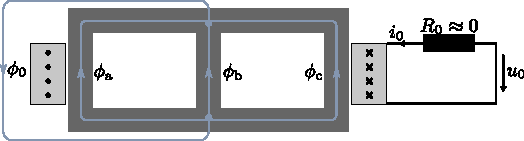
\includegraphics[width=0.7\textwidth]{fig/lec04/Zero_flux_model.pdf}
		\caption{Substitute model to represent the zero flux component}
		\label{fig:Zero_flux_model}
	\end{figure}
\end{frame}


%%%%%%%%%%%%%%%%%%%%%%%%%%%%%%%%%%%%%%%%%%%%%%%%%%%%%%%%%%%%%
%% Three-phase transformer connection and winding types %%
%%%%%%%%%%%%%%%%%%%%%%%%%%%%%%%%%%%%%%%%%%%%%%%%%%%%%%%%%%%%%
\begin{frame}
	\frametitle{Three-phase transformer connection and winding types}
		Each side of a three-phase transformer can be connected in:
		\begin{equation*}
			\mbox{Y/y: star connection,}\quad \mbox{D/d: delta connection,}\quad \mbox{Z/z: zigzag connection.}
		\end{equation*}
		The winding nomenclature is as follows:
		\begin{itemize}
			\item First upper case letter: primary side (high voltage)
			\item Second lower case letter: secondary side (low voltage)
			\item Number ($0\ldots 11$): phase deviation between the primary and secondary side in $^\circ 30$ steps
			\item Optional: N/n for neutral connection of  high/low side.
		\end{itemize}

		\begin{figure}
			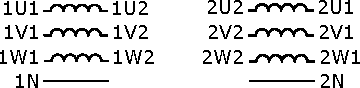
\includegraphics[width=0.45\textwidth]{fig/lec04/Connection_nomenclature_three_phase_transformer.pdf}
			\caption{Connection nomenclature of three-phase transformers}
			\label{fig:Connection_nomenclature_three_phase_transformer}
		\end{figure}
\end{frame}

%%%%%%%%%%%%%%%%%%%%%%%%%%%%%%%%%%%%%%%%%%%%%%%%%%%%%%%%%%%%%
%% Three-phase transformer connection and winding types (example: Dy11)%%
%%%%%%%%%%%%%%%%%%%%%%%%%%%%%%%%%%%%%%%%%%%%%%%%%%%%%%%%%%%%%
\begin{frame}
	\frametitle{Three-phase transformer connection and winding types (example: Dy11)}
	The transformer connection Dy11 indicates a delta connection on the primary side, a star connection on the secondary side, and a phase deviation of $330^\circ$ between the primary and secondary side.	
\end{frame}

%%%%%%%%%%%%%%%%%%%%%%%%%%%%%%%%%%%%%%%%%%%%%%%%%%%%%%%%%%%%%
%% Three-phase transformer connection symbols (vector groups) %%
%%%%%%%%%%%%%%%%%%%%%%%%%%%%%%%%%%%%%%%%%%%%%%%%%%%%%%%%%%%%%
\begin{frame}
	\frametitle{Three-phase transformer connection symbols (vector groups)}
	\begin{figure}
		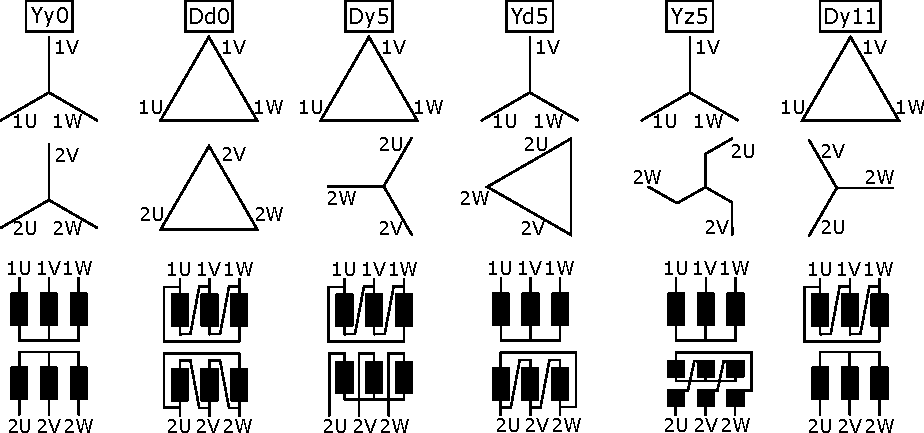
\includegraphics[height=0.75\textheight]{fig/lec04/Three_phase_transformer_connection_symbols_01.pdf}
		\caption{Exemplary connection symbols for three-phase transformers}
		\label{fig:Three_phase_transformer_connection_symbols_01}
	\end{figure}
\end{frame}